\documentclass{gifce}

% --- metadata section ----
%
% \gifceTitle, \gifceKeywords and \gifceAuthors are used both in PDF
% metadata and article typesetting
%
% \gifceShortTitle starts with the abbreviated first author's name.

\gifceTitle{Process isolation in PyWPS framework}
\gifceShortTitle{A. Laža}%
                {Process isolation in PyWPS framework}
\gifceKeywords{WPS; PyWPS; Docker; container; thread}
\gifceAuthors % {name}{affilation}{author ID (ORCID, Scopus, WoS)}{separator}
{
  \gifceAuthor{Ing. Adam Laža}{{a}}{}{}\\
  \gifceAuthor{Ing. Martin Landa, Ph.D.}{{a}}{}{}
}
% --- end of metadata section ---

%\gifceYear{2016}
%\gifceVolume{15}
%\gifceIssue{2}
%\gifceChapterNumber{3}
%\gifceChapterPage{27}
%
\pdfstringdefDisableCommands{\def\\#1{ #1}}
\hypersetup{
  pdftitle={\gifcejournalTitle},
  pdfsubject={Geoinformatics FCE CTU
    \gifcejournalVolume(\gifcejournalIssue), \gifcejournalYear},
  pdfauthor={\gifcejournalAuthors},
  pdfkeywords={\gifcejournalKeywords}
}
%
%
\gifceReleasefalse
\gifceNamestrue
\gifceWatermarktrue
%
\gifceConditionalWaterMark
\gifceResetAuthor
%
\addbibresource{gifce.bib}
%
%
\begin{document} %----------------------------------------------------------

% The review process is double-blind, information about authors must
% not be revealed to reviewers
%
% \gifcejournalShortTitle and \gifcejournalTitle are defined in the
% metadata section above

\begin{raggedright}\hyphenpenalty=10000 % ----------------------------------
\chapter[\gifcejournalShortTitle]{\gifcejournalTitle}
%
\ifgifceNames
%
  \gifcejournalAuthors

  \gifceAffiliation{a}\emph{%
  GeoForAll Lab,
  Department of Geomatics,
  Czech Technical University in Prague, Czech Republic}\\
\fi
\end{raggedright} %---------------------------------------------------------


\begin{abstract}
In order to process data independently of the type of
acquisition, format or platform, international standard interfaces and standardized
%% ML: nechybi v te druhe vete sloveso?
%% AL: neprijde mi. "Rozhrani a standard. frameworky jsou nezbytne."
frameworks are necessary. The Open Geospatial Consortium, Inc. (OGC) - an
organization oriented toward open geospatial standards - researches and establishes
technical standards for data compatibility and interoperability.
Besides quite famous and used standards as WMS and WFS, there exists the WPS
standard. The WPS standard defines an interface that facilitates the publishing of
geospatial processes. There
are several implementations of WPS standard. This article is focused on
the PyWPS - a WPS implementation written in Python - and its process isolation via Docker
technology. This Docker extension was developed during work on Master thesis that was 
defended in February 2018.
\end{abstract}
%
% keywords are added automatically from metadata


\section{Web Processing Service}

% All articles published in Geoinformatics FCE CTU have BibTeX records
% in the file `gifce.bib'. Keys are `gi.volume.number' for older issues or
% newly `gi.volume.issue.number' for articles published starting from
% volume 14.
%
% Authors citation records can have arbitrary keys and the cirresponding
% BibTeX records are placed in a single file (gifce-example.bib here).
%
% References are generated authomatically by `biber' for cited works, see
%
%      \printbibliography[heading=subbibliography]
%
% command atd the end of this example.
%
%
% In most of bibliography databases it is possible to generate BibTeX
% format citations (http://search.crossref.org/), great tool is zotero
% (https://www.zotero.org/), ISBN to BibTeX format convertor is
% availabel online at http://www.ottobib.com/.

The OGC Web Processing Service (WPS) Interface Standard defines a standardized interface
that facilitates the publishing of geospatial processes. Also provides rules how to standardize
requests and responses for geospatial processing services \cite{WPS_standart_1.0}. 

\textit{Process} means any operation on spatial
data from simple ones like maps overlay or buffering to highly complex as complicated global models. Any kind of GIS 
functionality can be offered to clients across a network with correctly configured WPS. 

\textit{Publishing} means
creating human-readable metadata that allow users to discover and use service as well as making 
available machine-readable binding information.

\textit{Data} can be both vector or raster data and can be delivered across the network or be available
at the server.

The interface does not specify any specific processes that can be implemented by a WPS nor any specific
data inputs or outputs. Instead it specifies generic mechanisms to describe any geospatial process and
data required and produced by the process. The interface does not only provide mechanisms for calculation
but also mechanisms that identify required data, initiate the calculation and manage output data so clients
can access it. 

\bigskip
Web Processing Service as one of the OGC web services specifies three types of requests which can be requested
by a client and performed by a WPS server. The implementation of these three requests is mandatory by all servers:

\textbf{\textit{GetCapabilities}} - The request returns to the client a Capabilities document that describes the abilities
of the specific server implementation. It also returns the name and abstract of each of the processes that can
be run on a WPS instance.

\textbf{\textit{DescribeProcess}} - The request returns details about the processes offered by a WPS instance. 
It describes required inputs and produced outputs and their allowable formats.

\textbf{\textit{Execute}} - The request allows the client to run a specified process with provided parameters and returns
produced outputs.


\subsection{PyWPS}
The origin of PyWPS started in 2006 as a student project. 
In 2007 PyWPS 2.0.0 was released supporting WPS standard 0.4.0. New
version improved stability and approached on the standard
implementation. It came with new WPS client and WPS plugin for
OpenLayers \footnote{\url{http://openlayers.org/}}.

Next year in 2008 PyWPS 3.0.0 was released with support for WPS 1.0.0. It was possible to run multiple WPS instances
with one PyWPS installation. This version had simple code structure and contained examples of processes. 
The newest version is PyWPS 4.0.0 from 2016. Rewriting from scratch involved these major changes:
\begin{itemize}
\item It is written in \textit{Python 3} with backward support for Python 2.7.
\item It utilizes native Python bindings to existing projects (GRASS GIS).
\item New popular formats like \textit{GeoJSON}, \textit{KML} or \textit{TopoJSON} are reflected and their support is provided.
\item PyWPS project has changed the license from \textit{GNU/GPL} to \textit{MIT}.
\item PyWPS 4.0 is implemented using the \textit{Flask} framework.
\item A C-based XML parser \textit{Lxml} is used to handle XML files.
\item \textit{OWSLib} structures are used for some data types.
\end{itemize}

\subsection{PyWPS-demo}
PyWPS-demo is a small side project distributed with PyWPS. It is a simple demo instance of PyWPS server running on 
\textit{Flask}\footnote{\url{http://flask.pocoo.org/}}. Flask is a microframework for web applications in Python. 
Flask provides built-in development server and debugger and RESTful request dispatching. PyWPS-demo comes with several demo processes such as \textit{area}, \textit{buffer}, \textit{centroids} and many others.

\section{Process isolation in PyWPS}
\subsection{Asynchonous requests}
Right now in PyWPS 4.0 version a PyWPS server instance is able to run
multiple concurrent processes in parallel. The server is configured
for maximal amounts of concurrently running processes at the same time
and for maximum of waiting processes in a queue, to later
start their execution once new slots are available. If the new Execute
request is received and the maximal amount is exceeded, the request is
rejected and user is informed in response (see
Lst. \ref{lst:Isolation_rejected}).

%% ML: vyresit preteceni textu
%% AL: vyreseno
\begin{lstlisting}[basicstyle=\small,caption={Resource exceeded exception},label={lst:Isolation_rejected}]
<?xml version="1.0" encoding="UTF-8"?>
<ows:ExceptionReport xmlns:ows="http://www.opengis.net/ows/1.1">
    <ows:Exception exceptionCode="ServerBusy">
        <ows:ExceptionText>
            Maximum number of parallel running processes reached. 
            Please try later.
        </ows:ExceptionText>
    </ows:Exception>
</ows:ExceptionReport>
\end{lstlisting}

To facilitate the management of concurrent processes, process metadata
are stored into a local database. This database is used for logging
and saving waiting Execute requests in the queue and invoking them
later on. The database will also enable the implementation of
pausing, releasing and deleting running process. These features will
allow PyWPS to comply with WPS version 2.0.0 \cite{WPS_standart_2.0}.

\subsection{Current state}
Current version of PyWPS offers two solutions for running parallel processes: \textit{Multiprocessing}
and \textit{Job Scheduler Extension}.

\paragraph{Multiprocessing}
By default for  processes running in the background, the Python \textit{multiprocessing} module is used – 
this makes it possible to use PyWPS on the Windows operating system too.

The number of processes running in parallel is configirable by parameter \textit{parallelprocesses} of section \textit{server} in 
configuration file. In the Fig. \ref{fig:Diag_multiprocessing} two running processes are shown. A client sends an Execute request to
a server. Server sends back to the client an ExecuteResponse that \textit{Process1} (green in the figure) was accepted and starts its 
execution. During the execution the process updates its status. The interval of status updates depends on the code of the Process1.
Process1 must support status update otherwise it cannot be run in asynchronous mode.

\begin{figure}[h!]
\centering
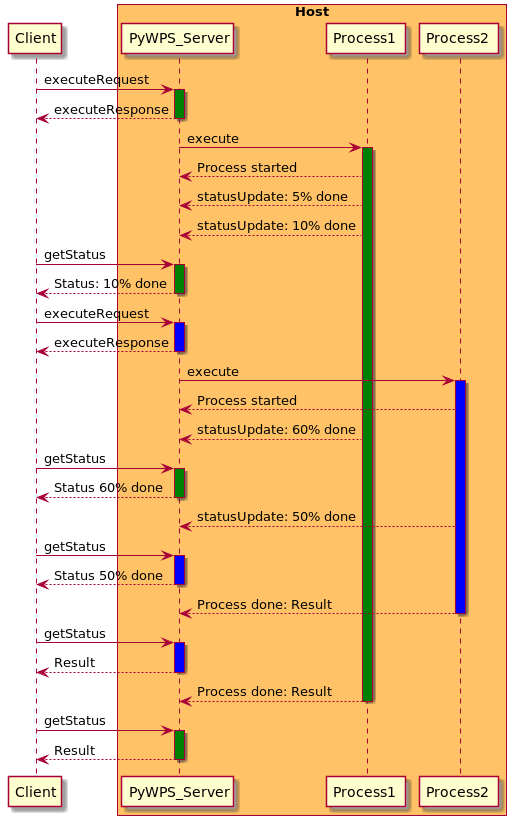
\includegraphics[width=0.5\textwidth]{img/Diag_multiprocessing.png}
%% ML: source: author
%% AL: pridano
\caption{Sequence diagram: Multiprocessing, source: author}
\label{fig:Diag_multiprocessing}
\end{figure}

During the execution of Process1 server receives another Execution request. It sends back the Execution response and starts the execution
of \textit{Process2} (blue in the figure). Separated Python \textit{Process} is created. Both of the processes run on the host machine, however both have own memory
space. Their executions run concurently and client can request their status. In the figure, the Process2 ended first and client can retrieve
the result from the server. Once the Process1 ends, the client can retrieve its result from the server as well.

It is important to say that in case of multiprocessing, processes run concurently with its own memory space, nevertheless they are not isolated.
They run on the same host machine and share the resources. There are even methods like \textit{Pipe()} that enable communication between 
processes.

\paragraph{Process vs Thread} In Python there are two ways to achieve \textit{pararellism}. It is \textit{multiprocessing}
\footnote{\url{https://docs.python.org/3/library/multiprocessing.html}} with using processes and \textit{threading}\footnote{\url{https://docs.python.org/3/library/threading.html}} with threads. The main difference is that threads run in the same memory space, while processes
have separate memory. Multiprocessing takes advantages of multiple CPUs and cores while threads are more lightweighted and have low memory
footprint. In case of PyWPS asynchronous requests, for every execution its own process with its own memory space is created.

\paragraph{Job Scheduler Extension}
PyWPS scheduler extension offers possibilities to execute asynchronous processes out of the WPS server machine.
This extension enables to delegate execution of processes to a scheduler system like \textit{Slurm}, \textit{Grid Engine} 
and \textit{TORQUE} from Adaptive Computing. These scheduler systems are usually located at \textit{High Performance Compute (HPC)}
centers.

\subsection{Possible solutions for process isolation}
In previous section there were described two mechanisms for running parallel processes. Nevertheless in case of Python module
\textit{Multiprocessing} the processes are not really isolated. They run concurrently but they can share resources and there are 
even methods like \textit{Pipe()} that enables communication between processes.

On the other hand \textit{Job Scheduler Extension} depends on
\textit{dill} library as well as on some external scheduler systems
like \textit{Slurm}, \textit{Grid Engine} or \textit{TORQUE}.

\bigskip
To isolate each process some other solutions were considered. 
Some were suggested by PyPWS developers with encouragement to make a feasible study. Others were discovered
during research on the internet forums like StackOverflow and few of
them were referenced in the documentation of other projects. After a short research, the Docker techonology
was chosen. The main reason was that this technology provides a mechanism for full isolation. Beside that
it also provides a mechanism for start/pause/stop process execution and this functionality
will be required to comply WPS 2.0.0 standard.

\section{Docker}
\textbf{Containerization} is a lightweight alternative to full machine virtualization. It involves encapsulating an application 
into a container with its own operating environment. It helps to run a containerized application on any physical machine without any
worries about dependencies. The origin of containerization lies in the \textit{LinuX Containers {LXC}} format. Containerization works only in Linux environments and can run only Linux applications.

\paragraph{Docker} is a Linux container technology that allows package and ship applications and everything it needs to
execute into a standard format, and run them on any infrastructure.

\subsection{Virtual machine vs. Docker container}
Both virtual machines and Docker containers are two ways how to deploy multiple, isolated applications on a single 
platform. They both offer a way to isolate an application and its dependencies into a self-contained unit that can run 
anywhere. They both offer some kind of virtualization. They differ in architecture, see Fig. \ref{fig:Docker_VM}, 
\ref{fig:Docker_container}.

\subsubsection{Virtual machine}
Let's start with a virtual machine (Fig. \ref{fig:Docker_VM}) and its layers description from the bottom up:

\begin{figure}[h!]
\centering
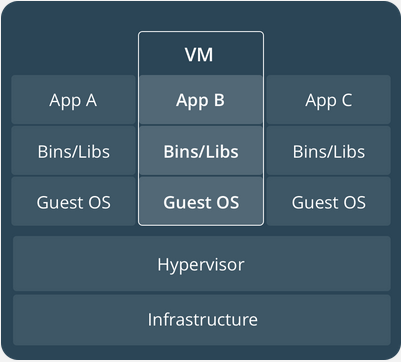
\includegraphics[width=0.4\textwidth]{img/Docker_VM.png}
\caption{Virtual machine architecture, source \cite{Docker_docs}}
\label{fig:Docker_VM}
\end{figure}

\begin{itemize}
\item \textit{Infrastructure} - It can be a PC, developer's laptop, a
  physical server in datacenter but as well a virtual private server
  in the cloud as Microsoft Azure or Amazon Web Services.
\item \textit{Host OS} - Host operating system. In case of native
  hypervisor this layer is missing. In case of hosted hypervisor it is
  probably some distribution of Linux, Windows or MacOS.
\item \textit{Hypervisor} - Also called virtual machine monitor (VMM). It allows hosting several different virtual machines
on a single hardware. There are two types of hypervisors:

\begin{itemize}
\item Type 1 -  Also called \textit{bare metal} or \textit{native}. This type is run on the host's hardware to control it as well as manage 
the virtual machines on it. It is much faster and more efficient. This type hypervisors are KVM, Hyper-V or HyperKit.
\item Type 2 - So called \textit{embedded} or \textit{hosted} hypervisors. These hypervisors are run on a host OS as a software. They are slower
and less efficient on the other hand they are much easier to set up. It includes VirtualBox or VMWare Workstation.
\end{itemize}
\item \textit{Guest OS} - Guest operating system. Each VM requires own guest operating system which is controlled by the hypervisor. Each 
guest OS needs its own CPU and memory resources and starts on hundreds of megabytes in size.
\item \textit{Bins/Libs} - Each guest OS needs various binaries and libraries for running the application. It can be \textit{python-dev} or \textit{default-jdk} packages as well as personal packages to run the application.
\item \textit{Application} - The application source code that is desired to be run isolated. Therefore each application or each version of the application has to be run inside of its own guest OS with own copy of bins and libs. 
\end{itemize}



\subsubsection{Docker container}
\noindent
Now, what is different regarding containers (Fig. \ref{fig:Docker_container}):

\begin{figure}[h!]
\centering
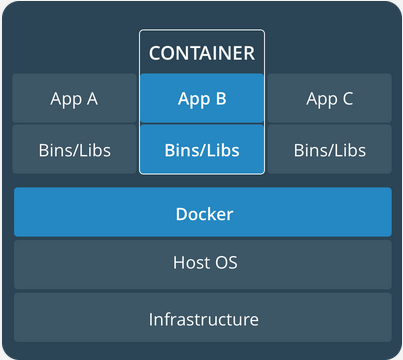
\includegraphics[width=0.4\textwidth]{img/Docker_container.png}
% source: ?
%% AL: pridano
\caption{Container architecture, source \cite{Docker_docs}}
\label{fig:Docker_container}
\end{figure}

\begin{itemize}
\item \textit{Infrastructure} - PC, laptop, physical or virtual server.
\item \textit{Host OS with container support} - Any OS capable of run Docker. All major distributions of Linux are supported and there are ways
to run Docker even on MacOs and Windows too.
\item \textit{Docker engine} - Also called Docker daemon. It is a service that runs in the background on host operating system. It manages all interaction with containers.
\item \textit{Bins/Libs} - Binaries and libraries required by the application. They get built into special packages called \textit{Docker images}.
The Docker daemon runs those images.
\item \textit{Application} - Each application and its library dependencies get packed into the same Docker image. It is managed independently by the Docker daemon. 
\end{itemize}

\noindent
But the architecture is not the only one difference:
\begin{itemize}
\item Docker uses Docker daemon to manage containers, hypervisor manages virtual machines.
\item The Docker daemon communicates directly with host OS and manage resources for each container.
\item VMs usually boot up in a minute and more, containers start in seconds.
\item Docker virtualizes operating systems, using VMs is hardware virtualization.
\item VM and container vary in size. VMs start at hundreds of megabytes. A container can be smaller than one megabyte.
\item Containers share the kernel although they are isolated. VMs are monolithic and stand-alone.
\end{itemize}

\subsection{Dockerfile}
Dockerfile is a core file that contains the instruction to be performed when an image is built. It usually consists of commands to install packages, calls to other scripts, setting environmental variables, adding files or setting permissions. In Dockerfile there is also defined what image is to be used as a base image for the build.

\section{Implementation}
The implementation of the Docker extension was realized during
the work on a Master thesis \cite{thesis}. The goal was to get
the extension into the main develop branch of PyWPS project.

\subsection{pywps-demo}
During the implementation the \textit{pywps-demo}
running on \textit{Flask} framework was
used. This demo server instance runs on host machine server at port
5000 as well as the image built from its Dockerfile is used for every
container creation. For developing purpose some sections were added to
configuration file as well some minor changes for instance in server
routing were made.

\subsubsection{pywps-demo Dockerfile}
\textit{pywps-demo} is also available as a Dockerfile and as mentioned
the image built from this Dockerfile is used for container creation.
%% ML: nahradit thesis za jine slovo...
%% AL: nahrazeno
Before the Docker extension was added, the pywps-demo project had
offered two dockerfiles, both based on \textit{Alpine Linux}
distribution. The first one \textit{pywps-flask} was the default
implementation using only Flask while the second one \textit{nginx}
implements PyWPS using Nginx and Green unicorn as WSGI server. During
the implementation only the \textit{pywps-flask} Dockerfile was
used. However it was necessary to modify the Dockerfile because it did
not contain \textit{GDAL} library which is required for most of the
demo processes that \textit{pywps-demo} offers. This Dockerfile modification
was realized in collaboration with PyWPS developers.
%% ML: Prvni vetu prepis, nedava prilis smysl
%% AL: upraveno
%% ML: Posledni vetu vynech, jde zbytecne do detailu
%% AL: Smazano.
developers.

\subsection{OWSLib}
\label{sub:owslib}
A Python package \textit{OWSLib} was used for forwarding requests from
PyWPS server instance running on host machine to PyWPS server instance
running inside a Docker container. Some bug fixing was necessary\footnote{Pull request at: \url{https://github.com/geopython/OWSLib/pull/410}}.

\subsection{PyWPS}
Most changes have been done in core PyWPS project. Almost all changes were made in \textit{processing} module. To this module new file \textit{container.py} containing the \textit{Container} class was added.

\section{Execute operation}
\label{sec:operations_ov}
PyWPS in current version 4.0.0 implements all mandatory operations: \textit{Execute}, \textit{GetCapabilities}, \textit{DescribeProcess}.
Operations are handled by corresponding methods \textit{execute()}, \textit{get\_capabilities()} and \textit{describe()} in \textit{Service} class. 

However both \textit{GetCapabilities} and \textit{DescribeProcess}
operations run in synchronous mode only. After sending a request, a
client receives back GetCapabilities or DescribeProcess response and
\ref{para:DesribeProc_response}). Both operations return only
information or description about process but do not trigger the
execution of the process. It is supposed the response to
GetCapabilities and DescribeProcess is returned almost immediately.
During the GetCapabilities and the DescribeProcess operations a
process execution is not started and therefore there is no starting
process to be isolated. That is why whole contribution
only applies to \textit{Execute} operation.

\subsection{Process.execute()}
The method \textit{execute()} of class \textit{Process} contains crucial if-statement where is decided whether the process will be
run in asynchronous or synchronous mode. Running in asynchronous mode can be enforced by setting both attributes \textit{status} and \textit{storeExecuteResponse} of the \textit{ResponseDocument} element in the ExecuteRequest XML to True.

\begin{lstlisting}[basicstyle=\small,caption={ReponseForm element of ExecuteRequest XML},language=XML,label={lst:Execute_ResponseForm}]
<wps:ResponseForm>
 <wps:ResponseDocument status="true" storeExecuteResponse="true">
  <wps:Output asReference="true">
   <ows:Identifier>buff_out</ows:Identifier>
  </wps:Output>
 </wps:ResponseDocument>
</wps:ResponseForm>
\end{lstlisting}

No matter whether the process runs synchronously or asynchronously there is always a control how many parallel processes are currently
running. The number of the maximum of concurrently running processes can be configured. If the process is asynchronous and the number of currently running processes exceeds the maximal number, the process is stored and its execution is started lately. In case of the synchronous process the \textit{ServerBusy} exception is raised. If the number of processes is smaller than the maximal number of 
concurrent processes, the process can be executed. In synchronous mode the \textit{\_run\_process()} is called, in asynchronous mode the method \textit{\_run\_async()} is called. The activity diagram of the \textit{Process.execute()} is displayed in Fig.\ref{fig:Diag_process_execute}.

\begin{figure}[h!]
\centering
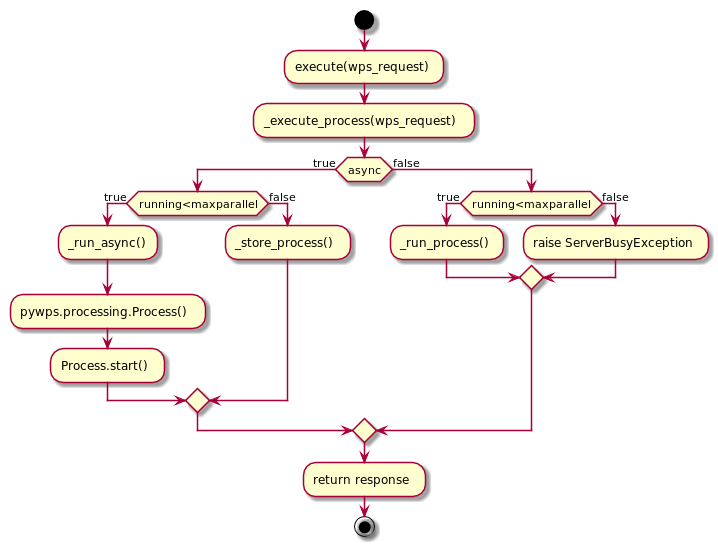
\includegraphics[width=0.6\textwidth]{img/Diag_process_execute.png}
\caption{\textit{Activity diagram: Process.execute()}, source: author}
\label{fig:Diag_process_execute}
\end{figure}

\subsection{Processing module}
As mentioned, PyWPS uses solely the Python package \textit{Multiprocessing} in production version.
In develop branch there is also \textit{Scheduler} extension as one of the option for multiprocessing. This article
describes another option for processing - \textit{Docker}. The desired option for processing can be configured in configuration file via parameter \textit{mode} in section \textit{processing}.

\section{\textit{Container} class}
The whole Docker implementation is in \textit{Container.py} module. The class \textit{Container} handles containers creation, interaction with server, file-system mounting and all container management.

The main idea of process isolation using Docker is quite simple. For every process execution one separate Docker container is created.
Instead of starting process execution on the host PyWPS server after receiving ExecuteRequest from the client, the ExecuteRequest is
forwarded to PyWPS server running inside Docker container. The process execution runs inside the container. After successful process
execution the outputs are available at the host server. The host server and the container share the same process workdir at filesystem.

\begin{figure}[h!]
\centering
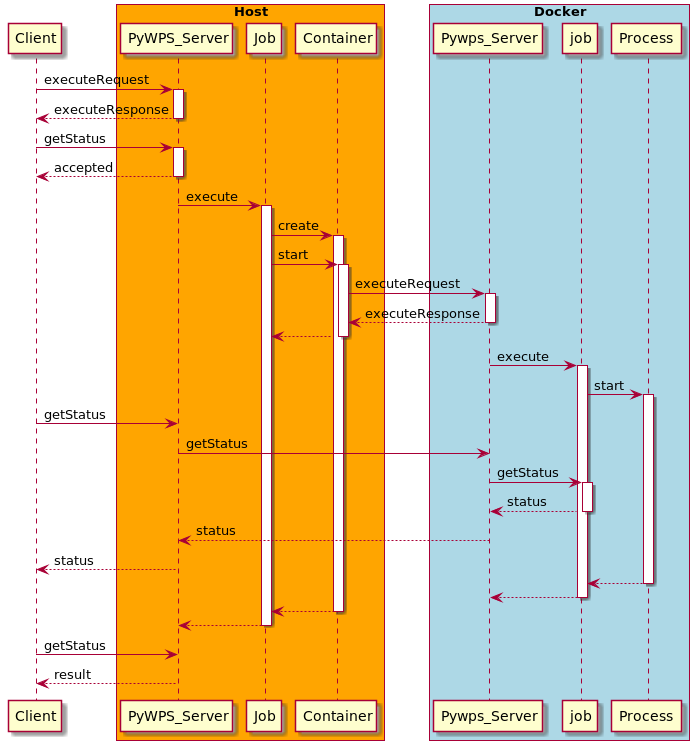
\includegraphics[width=0.6\textwidth]{img/Diag_sequence.png}
\caption{Sequence diagram: Process execution using Docker, source: author}
\label{fig:Diag_sequence}
\end{figure}

The method that creates a separate container for each takes as a parameter a dictionary
that defines ports to bind inside the container. The keys of the
dictionary are the ports to bind inside the container (port 5000
inside \textit{Container 1} and \textit{Container 2} at
Fig. \ref{fig:Diag_port}). The values of the dictionary are the
corresponding ports to open on the host (port 5050 for \textit{Job1},
port 5051 for \textit{Job2} at Fig. \ref{fig:Diag_port}).

\begin{figure}[h!]
\centering
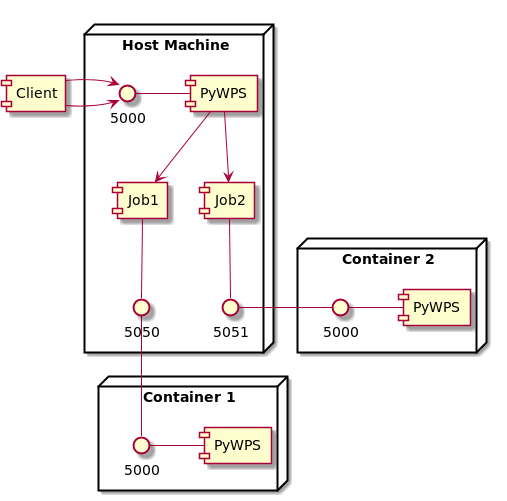
\includegraphics[width=0.45\textwidth]{img/Diag_ports.png}
\caption{Ports assignment schema, source: author}
\label{fig:Diag_port}
\end{figure}

Another optional parameter is \textit{volumes}. It is a dictionary 
to configure volumes mounted inside the container. The key is the host path and the value is a dictionary with the keys: \textit{bind}
- the path to mount the volume inside the container, and \textit{mode} - either \textit{rw} to mount the volume read/write, or 
\textit{ro} to mount it read-only.

Every container created with defined parameters \textit{volumes} and
\textit{ports} will have output directory on the host mounted into the
container output directory as well as the process workdir at host
machine mounted into container directory with data. Therefore, all
inputs downloaded to process workdir will be available for the
container and all outputs produced after process execution will be
stored at host machine output directory. Displayed in
Fig. \ref{fig:Diag_mount}.

\begin{figure}[h!]
\centering
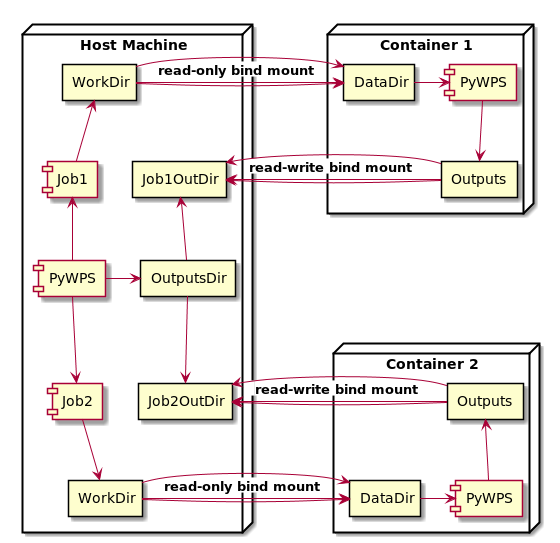
\includegraphics[width=0.45\textwidth]{img/Diag_mount.png}
\caption{Schema of mounting directories, source: author}
\label{fig:Diag_mount}
\end{figure}

To forward request from server to container \textit{OWSLib}
library (Sec. \ref{sub:owslib}) is used. OWSLib is a Python package for client programming with OGC web services 
interface standards.

\textit{WebProcessingService} object from OWSLib package is responsible for sending request to container. Its constructor takes URL of the
WPS server running inside container. Container URL varies depending on the port assigned to the container. Then the \textit{WPSExecution}
object is assigned to the \textit{Container} instance. The WPS\-Execution object is returned from \textit{WebProcessingService.execute()} 
method that takes process identifier, list of inputs and outputs as parameters.

The object \textit{WPSExecution} has \textit{statusLocation} property that contains path to XML file.
This file is updated several times during process execution so the client can check process execution progress.
After successfully finished execution, the XML file contains link to computed outputs.

At the server there run asynchronous daemon that cares about stopping and removing Docker container, removing
job workdir and temporary files. It prevents from accumulation of running but already unused Docker containers.


\begin{figure}[h!]
\centering
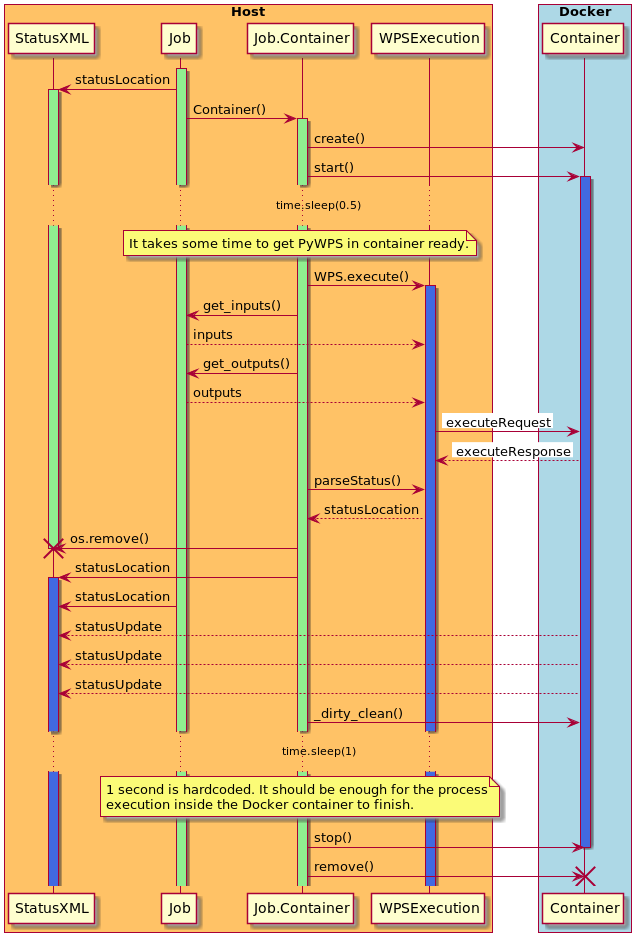
\includegraphics[width=0.5\textwidth]{img/Diag_WPSExecute.png}
\caption{Schema of \textit{WPSExecution}, source: author}
\label{fig:DiagWPSExecute}
\end{figure}


\section{Conclusion}

%% ML: diplomova prace by mela byt v referencich, citovat bys ji mohl
%% i drive nez v zaveru
%% ML: zaveru by neuskodilo rozsireni
This article is based on the master thesis. The goal of the thesis 
was to find and implement a solution for
process isolation in \textit{PyWPS}. This functionality was demanded
by PyWPS developers who would appreciate the possibility to isolate
each process execution. With every process fully isolated, a higher
level of security is ensured. Moreover, without the isolation the
processes have access to a file-system of a hosting OS.

But there are other reasons considered. One of them is a
performance. Non-isolated processes share the resources of a host
machine. In case that a client requests an execution of a process that
is poorly designed, its execution can consume a lot of resources and
thus it may slow down other process executions running in parallel. In
the worst-case scenario a process execution can bring down the server.

The reseach in the thesis covered various solutions for the process 
isolation. The functionality for the isolation was the main criterion, 
however beside that the selected solution should provide some mechanisms 
to control the execution of the process. These mechanisms will be 
necessary for implementation of the WPS 2.0.0 standard.

The \textit{Docker} Container Extension has been on the developers
wishlist for a long time. The container encapsulates the process
execution and also offers methods to start, pause, stop or kill the
container and thus the execution. Moreover using Docker opens
possibilities of Web Processing Service in a cloud computing
infrastructure.

The architecture is based on \textit{pywps-demo} project. It offers a
demo server instance of PyWPS. When a process execution is requested,
a server creates a Docker container with the demo server instance
running inside. The request is forwarded into the container. The
process execution runs inside the container but the container output
directory is mounted into the server file-system so the results are
available on the server.

The Docker extension was merged into the main develop branch of PyWPS project.
The text of the thesis and its source code,
are available at GitHub repository of this 
thesis.\footnote{\url{https://github.com/ctu-geoforall-lab-projects/dp-laza-2018/}}

\printbibliography[heading=subbibliography]
\cleardoublepage
\end{document} % -----------------------------------------------------------
